%%
%% ****** ljmsamp.tex 13.06.2018 ******
%%
\documentclass[
11pt,%
tightenlines,%
twoside,%
onecolumn,%
nofloats,%
nobibnotes,%
nofootinbib,%
superscriptaddress,%
noshowpacs,%
centertags]%
{revtex4}
\usepackage{ljm}
\begin{document}

\titlerunning{Short form of the title} % for running heads
\authorrunning{V. P. Kosyakov} % for running heads
%\authorrunning{First-Author, Second-Author} % for running heads

\title{Structural and Parametric Identification \\ of an Aquifer Model for an Oil Reservoir}
% Splitting into lines is performed by the command \\
% The title is written in accordance with the rules of capitalization.

\author{\firstname{V.~P.}~\surname{Kosyakov}}
\email[E-mail: ]{lik.24@yandex.ru}
\affiliation{Tyumen Branch of Khristianovich Institute of Theoretical and Applied Mechanics SB RAS, Taymirskaya Str. 74, 625026, Tyumen, Russia}


\received{March 02, 2020} % The date of receipt to the editor, i.e. December 06, 2017


\begin{abstract} % You shouldn't use formulas and citations in the abstract.
During the development modeling process of an oil reservior, one of the most important steps is to solve the inverse problem, the solution of which, as a rule, is to select the model parameters for the best mathcing to the development history. However, the purpose of modeling is not only to repeat development indicators on the historical period, but also to obtain a reliable forecast of the behavior of the simulated object in the future. Therefore, from the point of view of the long-term forecast characteristics of the model, it is necessary to perform not only parameter, but also structure identification of the model.
In this paper, an example of solving the problem of structure and parameter identification of an aquifer model for modeling the development of an oil reservoir is a study of predicted characteristics. It is shown that, as a result of structure and parameter identification of the model, its predictive properties can be significantly improved compared with the case of conventional parameter identification.
\end{abstract}

\subclass{76S05, 90C31} % Enter 2010 Mathematics Subject Classification.

\keywords{inverse problem, structure and parameter identification, numerical modeling, aquifer} % Include keywords separeted by comma.

\maketitle

% Text of article starts here.

\section{Introduction}

In the process of modeling the development of an oil field, one of the most important steps is to solve the inverse problem, which, as a rule, consists in selecting the model parameters for the best adjustment to the development history. In turn, the purpose of modeling is not only to repeat development indicators on the historical period, but also to obtain a reliable forecast of the behavior of the simulated object. The choice of a mathematical model is determined by the goals and objectives for the solution of which it will be used. In this case, the goal is to obtain a quality forecast. Based on the requirements of history matching and forecasting problems, the identification problem consists in determining the structure and parameters of a mathematical model that provide a satisfactory description of historical data and have the best predictive characteristics.

To assess the predicted characteristics of the model, a breakdown of the historical period into 2 time intervals is often used: on the first, the model is matched, and on the second, the forecast properties of the model are evaluated. It was shown in \cite{mus} that the best history matching does not necessarily have the best predictive properties, which largely depend on the complexity of the chosen model. In addition, the predicted characteristics depend on the specific conditions (control parameters) of the model at the stages of history matching and validation.

This paper presents a study of the dependence of the predicted characteristics of the model on the consistency of operating modes at the stages of adaptation and validation. Using the structure and parameter identification of an aquifer model for an oil field as an example, the importance of structural identification for the long-term predictive characteristics of the model is shown. The reservoir pressure, which characterizes the "energy" potential of the reservoir, acts as a predicted parameter. The choice of an aquifer model is important for obtaining acceptable predictive characteristics from the point of view of the energy state of the development object. In conditions of intensive development of the \cite{kos} reservior, which includes exploitation in the depletion mode, drilling new wells, the formation of a system for maintaining reservoir pressure, massive shutdown of wells, etc. a change in reservoir pressure can be significant.

\section{MATHEMATICAL MODELS}
To solve this problem, a two-dimensional mathematical model of single-phase filtration of a weakly compressible fluid was used as a filtration model \cite{bas}.
\begin{equation} \label{fil}
\triangledown\sigma\triangledown P = \beta^*h\frac{dP}{dt}+\delta(x,y),
\end{equation}
\begin{equation} \label{bc}
\delta(x,y)  = \left\{\begin{array}{crl}
0, \;\mbox{if}\;(x,y) \notin\ \Gamma_{in}\cup\Gamma_{out}\\
q_j, \;\mbox{if}\;(x,y) \in \Gamma_{in}\\
q_{aq}, \;\mbox{if}\;(x,y) \in \Gamma_{out}
\end{array}\right.,
\end{equation}
\begin{equation*}
P = P_0\mbox{,\quad if $t=0$},
\end{equation*}
where $\sigma$ is hydraulic conductivity, $P$ is reservoir pressure, $\beta^*$ is effective compressibility, $h$ is effective thickness, $q_j$ is fluid flow in $j$ well, $\Gamma_{in}$ is the set of coordinates of sources/drains (wells), $\Gamma_{out}$ is the external boundary, $P_0$ is the reservoir pressure at the initial instant $t=0$, $q_{aq}$ is the specific fluid flow through the external the border, which is according to the formula:

\begin{equation} \label{qaq}
q_{aq} = \lambda\sigma(P|_{\Gamma_{out}}-P_{aq}),
\end{equation}
\begin{equation*}
P_{aq} = P_0\mbox{,\quad if $t=0$},
\end{equation*}
where $P_{aq}$ is the mean pressure in the aquifer, $\lambda$ is the aquifer productivity coefficient.

To close the equations (\ref{fil}) - (\ref{qaq}), the model of the aquifer contour is used, which in general can be represented as:
\begin{equation} \label{f_aq}
F(P_{aq}, P,\boldsymbol{\nu})=0,
\end{equation}
where $\boldsymbol{\nu}$ is a set of adjustable parameters of the aquifer, the composition of which depends on the complexity of the model. The calculations used 4 models of varying degrees of complexity \cite{dake}, \cite{fet}. As models of the aquifer were used:

\textbf{\textit{Isolated object.}}
Model (M1) describing the behavior of an isolated object. There is no fluid flow through the external boundary $\Gamma_{out}$, the equation (\ref{qaq}) is replaced by:
\begin{equation}
q_{aq} = 0,
\end{equation}
the equation (\ref{f_aq}) is not used.

\textbf{\textit{Constant pressure in aquifer.}}
Model (M2) describes maintaining a constant pressure in the aquifer equal to the initial pressure (aquifer of infinite volume).
\begin{equation}
q_{aq} = \lambda \sigma (P|_{\Gamma_{out}} - P_c),
\end{equation}
where $P_c$ is the pressure on remote aquifer ($P_c = P_0$). It has one configurable parameter, $\boldsymbol{\nu} = [\lambda]$.

\textbf{\textit {Aquifer of finite volume.}}
Model (M3) allows us to describe the change in pressure $P_{aq}$ in an aquifer with a finite volume.
\begin{equation}
F(P_{aq}, P,\boldsymbol{\nu})=\beta^*V_{aq}\frac{dP_{aq}}{dt} - \lambda\oint_{\Gamma_{out}}\frac{\sigma}{h}(P-P_{aq})dl = 0,
\end{equation}
where $V_{aq}$ is the volume of aquifer. The model has 2 custom parameters, $\boldsymbol {\nu} = [\lambda, V_{aq}]$.

\textbf{\textit{Aquifer of finite volume with a remote aquifer.}}
Model (M4) aquifer the final volume with the remote
aquifer is recorded as follows:
\begin{equation}
F(P_{aq}, P,\boldsymbol{\nu})=\beta^*V_{aq}\frac{dP_{aq}}{dt} -\lambda\oint_{\Gamma_{out}}\frac{\sigma}{h}(P-P_{aq})dl - \kappa(P_c - P_{aq})=0,
\end{equation}
where $\kappa$ is the productivity of the remote zone. It allows to take into account the influx or outflow of fluid from the aquifer into a remote aquifer having a pressure of $P_{c}$. The M4 model has 3 parameters, the vector $\boldsymbol{\nu} = [\lambda, V_{aq}, \kappa]$.

For models M3 and M4, the effective compressibility for the aquifer is taken to be equal to the effective compressibility of the computational domain $\beta^*$.

A custom parameter $a$ was introduced into the filtration model (\ref{fil}) so that $\sigma = a\cdot \sigma_0$, where $\sigma_0$ is the initial approximation for hydraulic conductivity. Denote by the vector $\boldsymbol{u}$ the set of parameters that must be found as a result of the solution, where $\boldsymbol{u} = [a, \nu_{1}, ..., \nu_{i}], \quad i = 1 ... N _ {\nu} $, $ N_{\nu}$ - the number of components of the vector $\boldsymbol{\nu}$.

The inverse problem is solved in the optimization statement, which consists in minimizing the objective function $J$, which is the mean absolute percentage error (MAPE). The arguments of the objective function are the actual (measured) and calculated values of the reservoir pressure at the locations of the wells at specified points in time. The objective function characterizes the deviation of the calculated and actual pressure values and is written as follows:
\begin{equation} \label{mape}
J=\frac{1}{N}\sum_{i=1}^N{\left\vert\frac{p_c^i-p_f^i}{p_f^i}\right\vert}
\end{equation}
where $p_c^i$ is the calculated value of reservoir pressure, $p_f^i$ is the actual value, $i$ is the measurement number, $N$ is the number of measurements. The calculated values, in turn, depend on the parameters of the model $u_k$. The solution is found using the gradient optimization algorithm and consists in determining the set of model parameters corresponding to the minimum $J$ and satisfying the constraints in the form of inequalities:
\begin{equation*}
u_{k\;min}\leq\ u_k\leq u_{k\;max}, \quad u_k \in \boldsymbol{u},
\end{equation*}
$u_{k\;min}$ and $u_{k\;max}$ - minimum and maximum values for each parameter.

When using the gradient optimization method, it is necessary to find the gradient components of the objective function, which can be written in the following form:

\begin{equation}
\frac{\partial J}{\partial u_k} = \frac{1}{N}\sum_{i=1}^N sgn\left(\frac{p_c^i-p_f^i}{p_f^i}\right)\frac{\partial p_c^i}{\partial u_k}.
\end{equation}
To solve the optimization problem, it is necessary that each component of the gradient of the objective function tend to 0, which can be written as:
\begin{equation} \label{rp}
	 \frac{\partial J}{\partial u_k} \rightarrow 0
\end{equation}

The solution of the inverse problem (\ref{rp}) is found numerically by the iteration method. At each iteration, the direct problem (\ref{fil} - \ref{f_aq}) is numerically solved and the derivatives of the objective function are calculated by the custom model parameters \cite{opt}. The numerical solution was found by the control volume method for a two-dimensional unstructured difference grid using an implicit time scheme.

\section{CALCULATION RESULTS}
As an example, the inverse problem of structural-parametric identification for an oil field was solved. To solve the problem, a data set is required (the size of the computational domain, the location of the wells and the development indicators for the wells: fluid flow and pressure), which was obtained using a synthetic hydrodynamic model. These data acted as "actual" values.

The location of the wells is shown in the figure \ref{fig:map}, the dimensions are indicated in meters.

\begin{figure}
    \begin{minipage}[h]{0.69\linewidth}
      \center{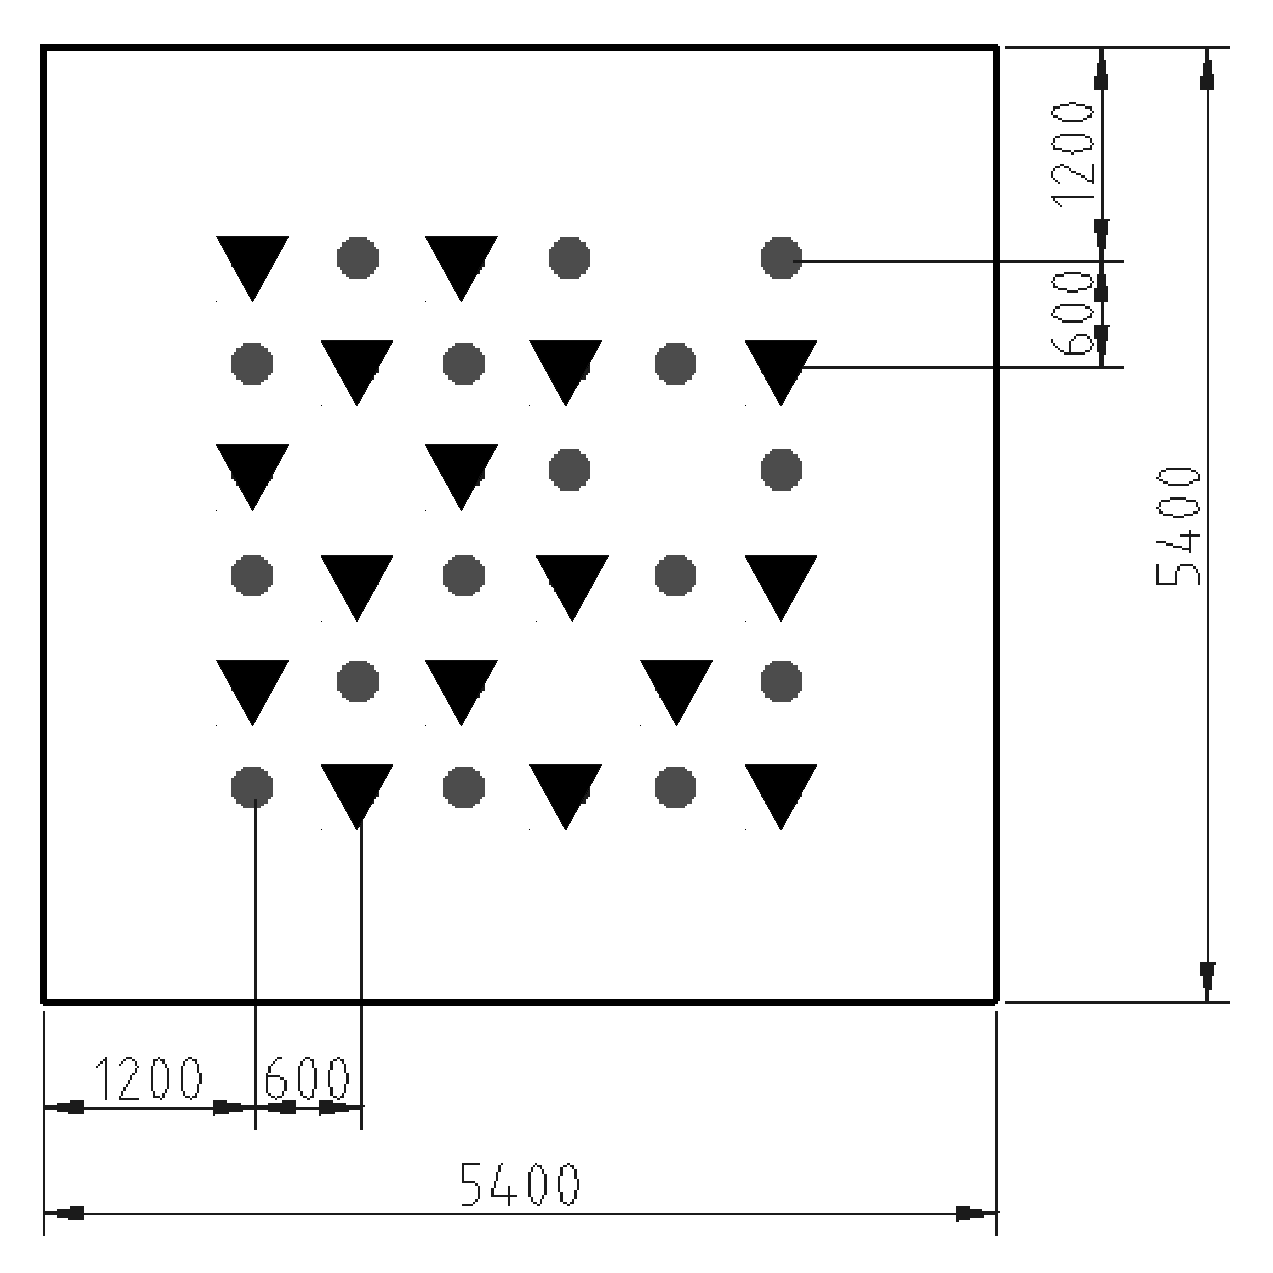
\includegraphics[width=20pc]{fig1a.eps}}
    \end{minipage} \hfill
    \begin{minipage}[h]{0.29\linewidth}
      \center{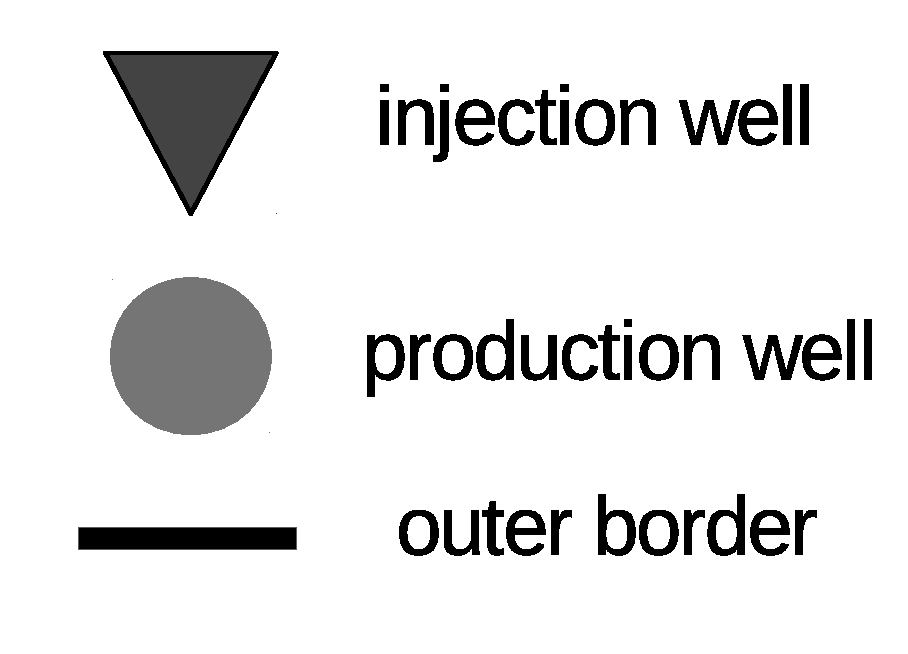
\includegraphics[width=8pc]{fig1b.eps}}
    \end{minipage} 
    \caption{Schematic representation of the computational domain.}
    \label{fig:map}
\end{figure}

TThe field is developed using 16 producing and 16 injection wells. The development period is 10 years, the power circuit was "connected" around the perimeter of the computational domain. To solve the problem of structural-parametric identification, the development period was divided into 3 intervals: 72, 24 and 24 months, respectively:
\begin{enumerate}
\item from 01-2000 to 12-2005 matching interval;
\item from 01-2006 to 12-2007 validation interval;
\item from 01-2008 to 12-2009 forecast interval.
\end{enumerate}

On the history matching interval, the inverse problem is solved for all 4 models; unknown parameters are found. On the validation interval, the predicted characteristics of the tuned model are evaluated, and the model with the best predicted characteristics is selected. Additionally, the 3rd interval was selected - the forecast interval, on which the behavior of the selected model is evaluated with a significant change in the control parameters. The time interval for the history matching phase was chosen so that it included the phased commissioning of all wells and a stationary mode of operation was achieved. The validation phase includes the period of stationary operation of the field.

For the forecasting phase, 3 operational scenarios were calculated for each model, and the behavior of the main development parameters was compared. The following scenarios were calculated: S0 is the stationary mode of operation in which the volume of injected fluid does not change, S1 is a twofold reduction in the volume of injected fluid, and S2 is a twofold increase in the volume of injected fluid compared to scenario S0.

Figure \ref{fig:din} shows the dynamics of the average reservoir pressure for the actual data (B is the base case) and aquifer models (M1-M4 aquifer models). The figure \ref{fig:hist} shows the values of the objective function (\ref{mape}) for the adaptation (adp) and validation (val) intervals, which characterizes the difference between the variant M1-M4 and variant B.
\begin{figure} 
    \begin{minipage}[h]{0.48\linewidth}
      \center{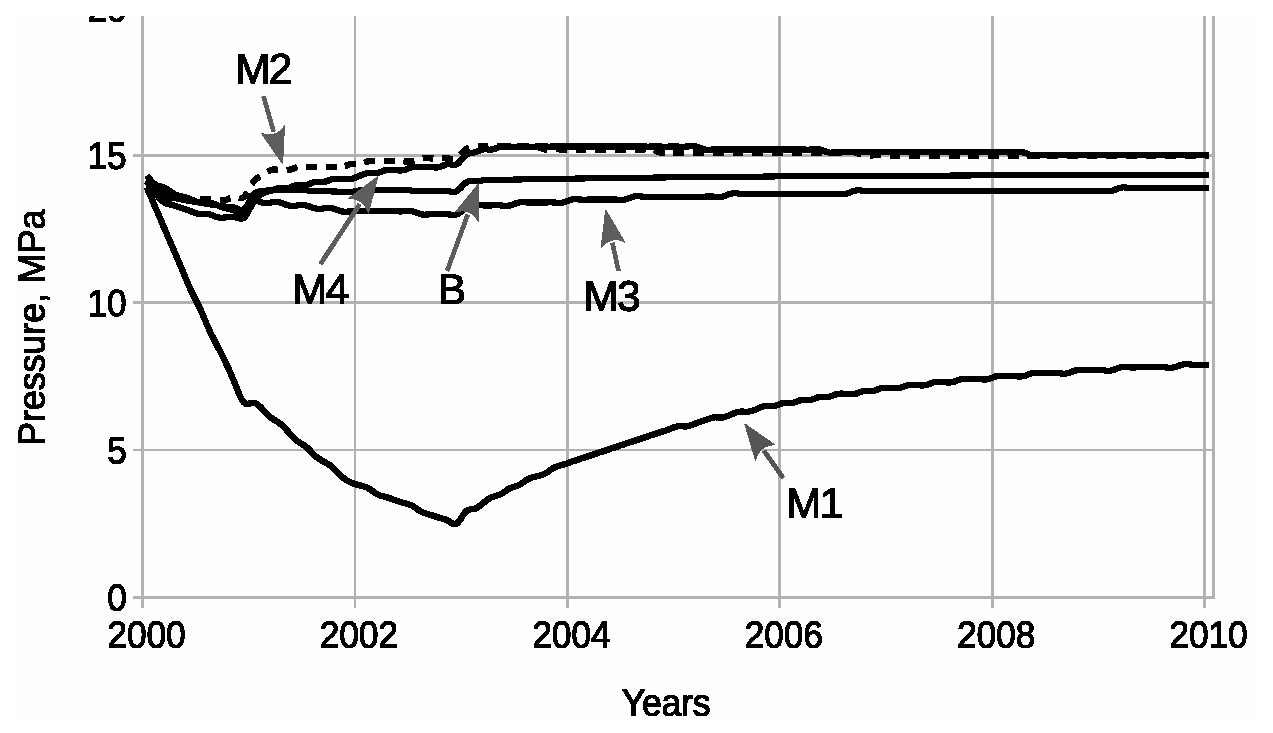
\includegraphics[height=0.60\linewidth]{fig2.eps}}
      \caption{Dynamics of the average reservoir pressure for different models of the aquifer}
      \label{fig:din}
    \end{minipage} \hfill
    \begin{minipage}[h]{0.48\linewidth}
      \center{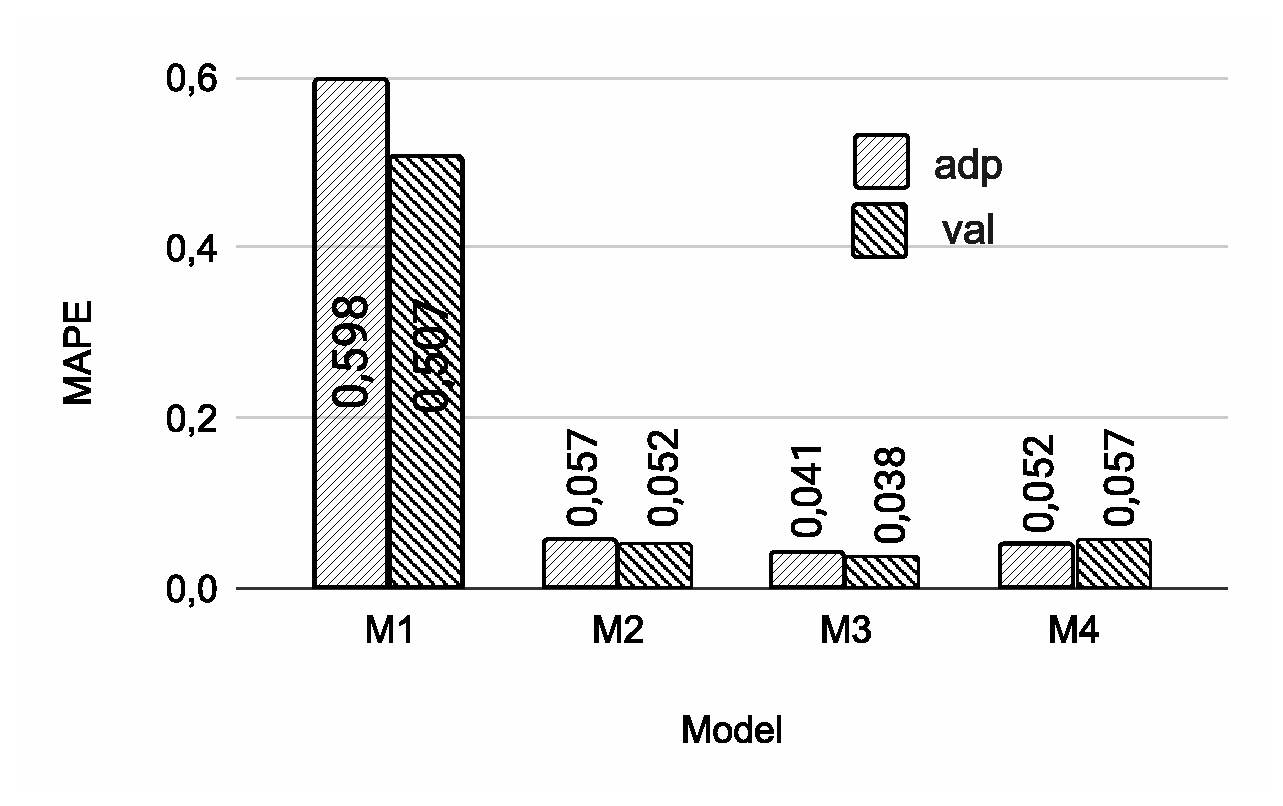
\includegraphics[height=0.60\linewidth]{fig3.eps}}
      \caption{MAPE for the adaptation (adp) and validation (val) stages}
      \label{fig:hist}
    \end{minipage} 
\end{figure}
It can be seen from the figures that the M1 model has the worst performance both at the adaptation stage and at the validation stage. The value of the objective function is approximately an order of magnitude greater than that of other models; therefore, the M1 model is the least suitable for describing the behavior of the modeled object and will not be used in further studies. The best characteristics for adaptation and validation are those of the M3 model. Models M2 and M4 have satisfactory values of the objective function. If you compare only these two models, then M4 describes the history better, and M2 has better predictive properties, respectively, the choice of these two models must be carried out using some other criteria, such as BIC \cite{mus}.

In practice, as a rule, only the adaptation problem is solved, and the choice of model is carried out expertly. Models are rejected mainly by the criterion of not exceeding the error inherent in various regulations (usually from 5 to 25\%). Correspondingly, the M2-M4 models, due to the relatively small difference in their indicators, can be equally likely selected as predictive models. Indeed, the most pronounced difference in pressure dynamics for different models is observed in the initial period - when new wells are entered and stationary wells are operating. In stationary modes, the models have close predictive characteristics.

The behavior of the adapted model with a significant (extreme) change in the operating mode of the wells, implemented in scenarios S1 and S2, is interesting. Figure \ref{fig:2din} shows the dynamics of the average reservoir pressure for three models (M2-M4) under three development scenarios (S0-S2).
\begin{figure}
\center{ 
    \begin{minipage}[h]{0.32\linewidth}
      \center{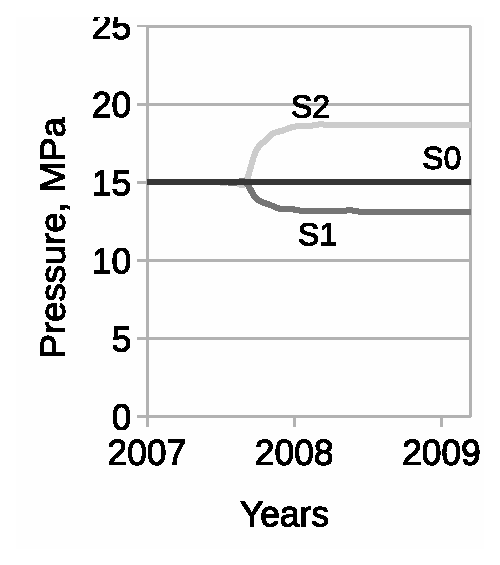
\includegraphics[height=0.95\linewidth]{fig4a.eps} \\ (a)}
    \end{minipage} \hspace{0pt}
    \begin{minipage}[h]{0.32\linewidth}
      \center{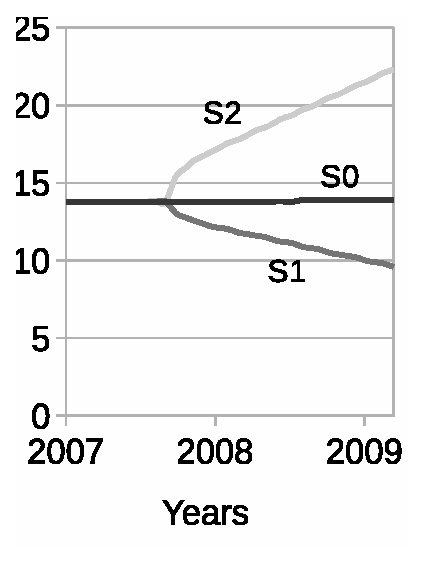
\includegraphics[height=0.95\linewidth]{fig4b.eps} \\ (b)}
    \end{minipage} \hspace{0pt}
    \begin{minipage}[h]{0.32\linewidth}
      \center{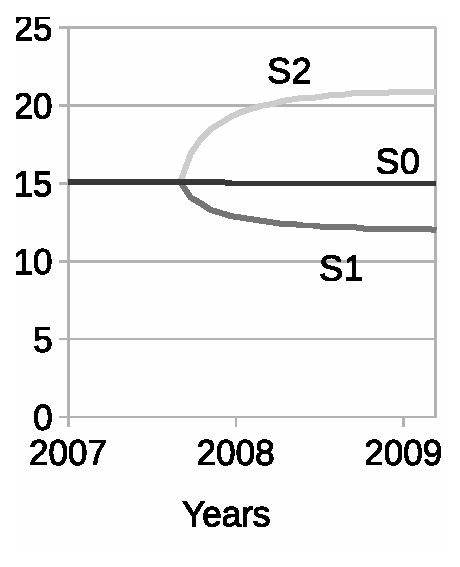
\includegraphics[height=0.95\linewidth]{fig4c.eps} \\ (c)}
    \end{minipage} 
    \caption{Dynamics of average reservoir pressure for 3 aquifer models under 3 development scenarios, where a, b, and c correspond to M2, M3, and M4.}
    \label{fig:2din}
    }
\end{figure}
As can be seen from the graphs, the behavior of the pressure curves under the same scenarios (S1 and S2) for different models are different. The difference lies not only in the values of reservoir pressure, but also in the dynamics of its change. Accordingly, the forecast indicators of each model will differ significantly. To maintain the predictive properties of the model within acceptable limits under significant changes in operating modes, the model updating procedure is necessary.

\section{CONCLUSIONS}

As a result of the study, it was shown that a satisfactory solution of the inverse problem can be obtained using models of varying degrees of complexity. In addition to the quality of tuning the model to the development history - the quality of adaptation, it is also necessary to evaluate its predictive properties. The validation procedure allows you to select the model that has the best predictive characteristics. In addition, the work demonstrated that the quality of prediction, in addition to the complexity of the model, depends on the development scenarios in which the model was matched and validated. With a significant difference between the predicted modes from those on which the model was tuned, the predicted properties of the model are sharply reduced. Upon receipt of evidence, it is necessary to re-carry out the procedure of structure and parameter identification.

\section{FUNDING}
The research was carried out within the framework of the Program of Fundamental Scientific Research of the state academies of sciences in 2013-2020 (project No. AAAA-A17-117030610130-1).


%
\begin{thebibliography}{99}
\bibitem{mus} E. N. Musakaev, S. P. Rodionov, D. Y. Legostaev, V. P. Kosyakov,  �Parameter identification for sector filtration model of an oil reservoir with complex structure� // AIP Conference Proceedings 2125,030113 2009;

\bibitem{kos} V. P. Kosyakov, D. Y. Legostaev,  �Computational technology for solution of the reverse problem of filtration theory for oil fields with an aquifer� // AIP Conference Proceedings 2125,030112 2009;

\bibitem{bas} K. S. Basniev, N. M. Dmitriev, R. D. Kanevskaya, V. M. Maksimov. \textit{Underground hydromechanics}. M.-Izhevsk: Institute for Computer Research, 2006. [in Russian]

\bibitem{dake} L. P. Dake, \textit{Fundamentals of Reservoir Engineering} (Elsevier, Amsterdam, 1978).

\bibitem{fet} M. J. Fetkovich. A Simplifi ed approach to water infl ux calculations ? Finite aquifer systems. J. Pet. Tech. July 1971, vol. 23, is. 7, pp. 814-828.

\bibitem{opt} V.P.Kosyakov, S.P.Rodionov "Optimal control of wells on the basis of two-phase filtration equations". Proceedings of MIPT. 2016. V. 8, N 3. P. 79?90.

\end{thebibliography}


\end{document}
